\documentclass[11pt,a4paper]{article}
\title{Next: preliminary results from first floor CAD}
\usepackage{cite}
\usepackage{hyperref}
\usepackage{textcomp}
\usepackage{amssymb}
\usepackage{subcaption}
\usepackage{amsfonts}
\usepackage{tabularx}
\newcommand{\norm}[1]{\left\lVert#1\right\rVert}
\usepackage[left=2cm,right=2cm,top=2cm,bottom=3cm]{geometry}
\usepackage{amsmath}
\setlength\parindent{0pt}
\usepackage{float}
\usepackage{placeins}
\pretolerance=10000
\tolerance=2000
\emergencystretch=10pt
\author{Lucy Henley, Joshua Moore, Timothy Ostler \& Thomas Woolley\footnote{moorej16@cardiff.ac.uk}}
\usepackage{graphicx}
\graphicspath{{./images_for_next/}}
\begin{document}
\maketitle

\section*{Key points}
\begin{itemize}
\item Based on the provided CAD file (titled `Front Building 1st.dwg', received 29/07/2020), we achieved a maximum seat occupancy, with a $2$m social distancing measure, of approximately $45\%$ without shielding, a significant improvement on the benchmark supplied at $28\%$.
\item We have developed a new web-based application which is specific to the Next first floor layout, available \href{https://lucyhenley.shinyapps.io/Next_seating/?fbclid=IwAR2Rx-OmoSkYHlw6BnQSKLgJGQt7VJvaX2IJYbqgKu4MK9YZxoZn1gBBAaEp}{here}. %The code can be found \href{https://github.com/Lucyhenley/Next_app}{here}.
\item A key assumption is that we are optimising only the number of available seats. This creates regions where people must walk through other people's `safety bubble' to access other facilities in the building.
\end{itemize}

\section*{What we could do next}
\begin{itemize}
\item Given the potential shield locations in the CAD file, we could simulate scenarios using shielding.
\item We can model other floors.
\item We can optimise our model to potentially return a greater seat occupancy.
\item We could refine our model to add in other factors, for example reducing exposure on walkways or incorporating the direction that desks are facing (a 1m social distance may be sufficient for people facing away from each other in the office).
\end{itemize}

\begin{figure*}[ht!]
\centering

\begin{subfigure}[h]{0.9\linewidth}
\centering
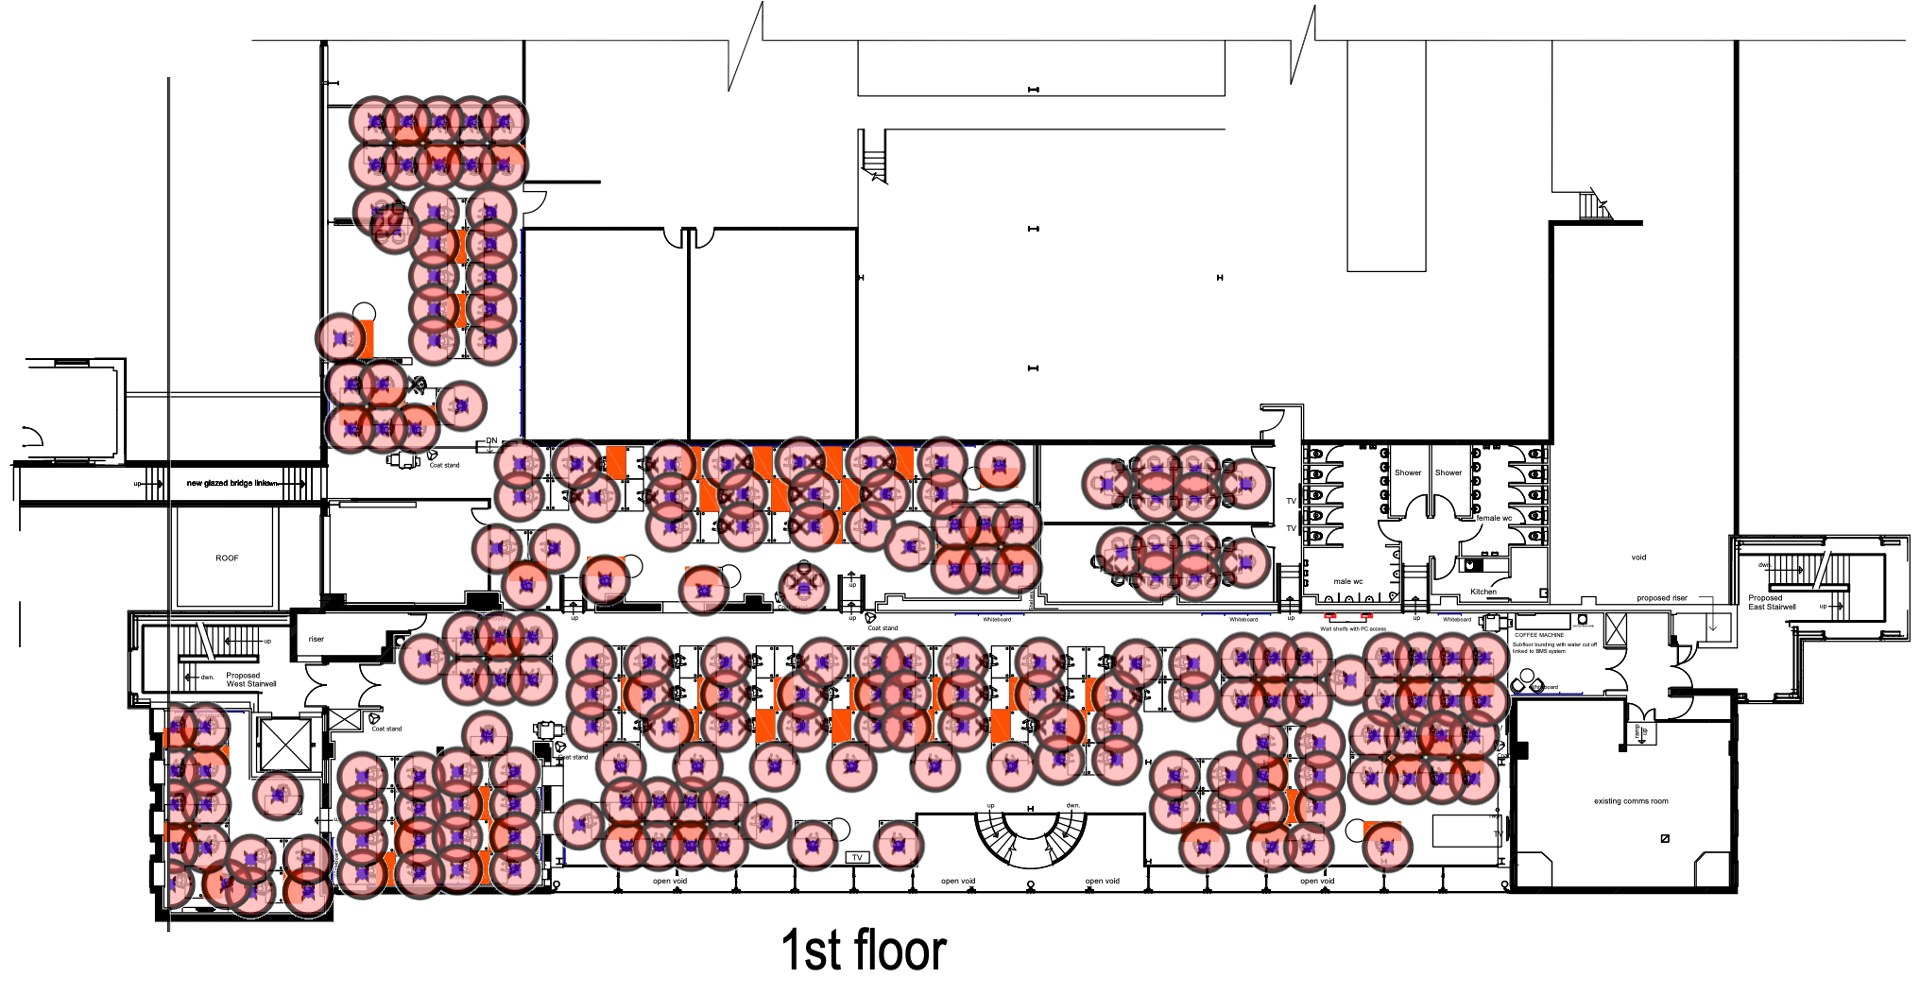
\includegraphics[width = \linewidth]{1m_overlay.png}
\caption{A sample layout for a social distancing measure of $1$ metres, which uses $201$ seats.}
\label{OneMetre}
\end{subfigure}
~
\begin{subfigure}[h]{0.9\linewidth}
\centering
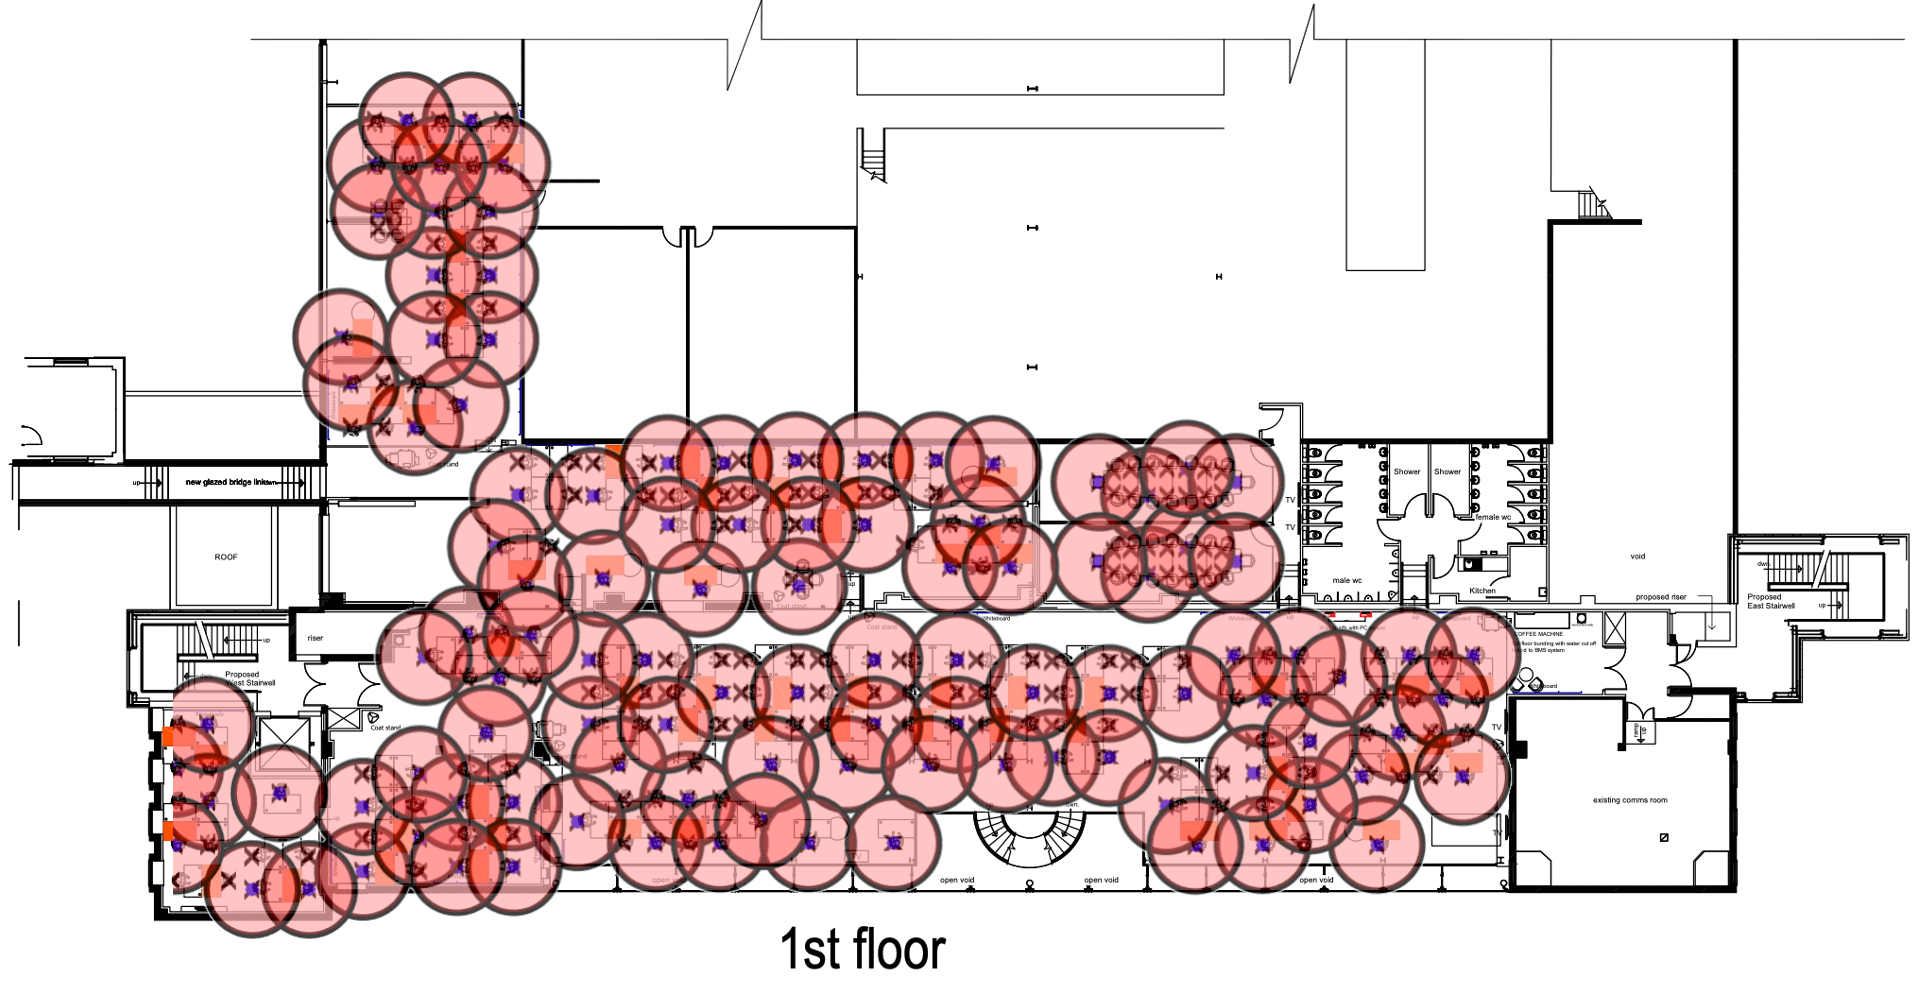
\includegraphics[width = \linewidth]{2m_overlay.png}
\caption{A sample layout for a social distancing measure of $2$ metres, which uses $105$ seats.}
\label{TwoMetre}
\end{subfigure}
\caption{A proposed office layout given by the app for $1$ and $2$ metre social distancing. Seat locations are marked with crosses, available seats are marked with dots and the `region of safety' is denoted by a circle around the available seats. Overlapping circles imply that certain regions are exposed to contamination from multiple sources, but no available seats are located in these regions. }
\label{Demonstration_pics}
\end{figure*}

\newpage

\section*{Methods and results}
Using the CAD file provided we reformatted the information to be compatible with our app. Upon selecting a fixed desk, the algorithm sweeps through all other seats and removes any desk that is within the social distance measure provided, repeating this process until all available desk spaces have been checked. In order to find an optimal solution, we simulated the desk selection randomly $5000$ times, selecting the order of fixed seats that yielded the greatest capacity. The results of the optimal desk selection algorithm are displayed in Figure \ref{Demonstration_pics} and in Table \ref{tab:performance}.  We have run simulations including and excluding the conference room.

%\begin{figure}[h]
    %     \centering
        % \includegraphics[width=1\textwidth]{random_order_sim.png}
        % \caption{Stochastic layout selection for the old building first floor, not including the conference room. Fixed desks are selected at random, then the algorithm sweeps through all desks and removes those too close to the accepted desks. The black line represents the capacity from each simulation, while the dashed red line corresponds to the mean of all simulations.}
    %     \label{fig:Stochastic_sims}
%\end{figure}






\begin{table}[ht!]
\begin{center}
 \begin{tabular}{|c |c|}
 \hline
& \textbf{Maximum capacity at $2$m social distancing (\%)}\\
 \hline
 Next CAD file benchmark &   27.9\\
 \hline
 Cardiff App  with conference rooms& 43.0\\
\hline
Cardiff App without conference rooms & 45.2\\
 \hline
\end{tabular}
\end{center}
\caption{Comparison of the performance of the Cardiff seat finding app against the benchmark provided in the supplied CAD file.}
\label{tab:performance}
\end{table}


As demonstrated in Table \ref{tab:performance}, we can very quickly achieve significantly higher occupancy rates in the office whilst maintaining social distancing measures. Given more time, we can search to see if our results can be further optimised and our model further improved, as well as develop methods for user specification of shield locations (see \href{https://lucyhenley.shinyapps.io/CardiffMATHBIO_NERCHackathonTwo_PublicTransport/}{first app}).

\section*{Prospective developments for improving optimality}
Our app always provides seating arrangements that maintains social distancing measures and provides locally optimal solutions which are already better than the $28\%$ benchmark provided. Returning the  absolute optimum arrangement is a lot more difficult because the problem is what is known as `NP-hard'.  Simply put, the only way to guarantee you have the most possible seats used is to try every possible order of seat checking, and pick the one which has the most seats used. Actually trying out every seat ordering would take a very long time; there are more ways to order $253$ seats than there are particles in the universe.\\

To improve our model, we could develop techniques to check our solutions and continuously improve upon them where possible. This would improve the likelihood we will find the best possible seating arrangement. For example, our current results are optimal up to $5,000$ simulations, however, this can extended with more computational power and further theoretical applications.\\


\subsection*{Costings for further work}
During this work, we established a new app which, currently, contains only the layout of the old office first floor. We reformatted the information from the CAD file so that it could interface with our app, and then ran our algorithm to determine a suitable seating plan. Further, we conducted a mathematical investigation of the problem to determine whether a true optimum is easily available, and then developed methods that could potentially improve on the first result found. In total, this work took approximately $2$ weeks to complete. An estimate of the number of hours and costing for this work is given in Table \ref{tab:costing_perfloor}. We estimate that repeating the analysis for further floors will require a similar number of hours, although this will depend on the number of desks on each floor.


\begin{table}[ht!]
\begin{center}
 \begin{tabularx}{\textwidth}{|X |l|l|}
%\begin{tabular}{|c |c|c|}
 \hline
\textbf{Task} &\textbf{Estimated time (hours)} &\textbf{Cost at £30 per hour} \\
 \hline
Extract seating layout from CAD file & 4 & £120 \\
\hline
Implement optimisation algorithm  & 8 & £240 \\
\hline
App development and integrating the seating layout & 8 & 240 \\
\hline
\textbf{TOTAL}  & 20 & £600 \\
\hline
\end{tabularx}
\end{center}
\caption{Estimated costing per floor for optimising seating layouts.}
\label{tab:costing_perfloor}
\end{table}

For further optimisation and extra measures to reduce risk, we will need to develop new algorithms. Estimates for the number of hours we expect for each of our suggested measures are given in Table \ref{tab:costing_extras}.


\begin{table}[ht!]
\begin{center}
 \begin{tabularx}{\textwidth}{|X |l|l|}
%\begin{tabular}{|c |c|c|}
 \hline
\textbf{Task} &\textbf{Estimated time (hours)} &\textbf{Cost at £30 per hour} \\
 \hline
Further optimisation of the seating algorithm to search for solutions with greater occupancy & 8 & £240 \\
\hline
Incorporate potential shield locations to further improve occupancy & 18 & £540 \\
\hline
Include the direction of desks, allowing for smaller social distancing between people facing away from one another & 18 & £540 \\
\hline
Reduce exposure on walkways by reducing the number of desks used at the edges of walkways  & 18 & £540 \\
\hline
\textbf{TOTAL}  & 62 & £1860 \\
\hline
\end{tabularx}
\end{center}
\caption{Estimated costing for possible future work to further improve occupancy rates.}
\label{tab:costing_extras}
\end{table}



\end{document}
